\problemname{Garden Decorations}

Every day when going to school and back home, Detje walks along a street with $N$ houses, numbered from $0$ to $N-1$.
Currently, house $i$ is inhabited by person $i$.
For a change of scenery, the residents have decided to switch houses with each other.
The person who will be moving into house $i$ is person $a_i$ (who currently lives in house $a_i$).

Each house has a bird statue in the garden.
The statues have two possible states; their wings are either \textit{open} (as if the bird is flying) or \textit{closed} (as if it is standing on the ground).

The residents have very strong preferences on how their bird statues should look.
Currently, the bird in front of house $i$ is in the preferred state of resident $i$.
Residents refuse to move to a house unless its statue is set to their preferred setting.
Detje wants to help them arrange the bird statues so they can move.

For this, she does the following: whenever she walks along the street (either on her way to school or back home),
she observes the birds she passes one by one and possibly adjusts some of the statues (by opening or closing their wings).
Since her days at school and at home are very busy, \textbf{she does not remember the states of the birds she saw on her previous walks}.
Luckily, she has written down the list $a_0, a_1, \ldots, a_{N-1}$, so she knows which resident is moving where.

Help Detje design a strategy that tells her which birds to manipulate in order to adjust the statues to the residents' likings.
She can walk along the street at most $60$ times, but to achieve a higher score, she should walk along the street fewer times.

\section*{Implementation}
This is a multirun problem, meaning that your program will be executed multiple times.

In each run, you should first read a line with two integers, $w$ and $N$, the index of the walk and the number of houses.
In the first run of your program $w = 0$, in the second $w = 1$, and so on (more details are explained below).

On the second line of input there are $N$ integers $a_0,a_1,\ldots,a_{N-1}$, meaning that
the person who will be moving into house $i$ is currently living in house $a_i$.
The $a_i$s form a \textit{permutation}: that is, each number from $0$ to $N-1$ appears exactly once in the list of $a_i$s.
Note that a resident can choose not to move; that is, $a_i = i$ is allowed.

The residents only switch houses once.
This means that for a fixed test case, the value of $N$ and the list of $a_i$s will be the same for all the runs of your program.

\paragraph{First Run.}
For the first execution of your program, $w = 0$.
In this run, you should simply output a single integer $W$ ($0 \le W \le 60$), the number of times you want Detje to walk past the houses.
Your program should then exit. Following this, your program will be executed again $W$ more times.

\paragraph{Subsequent Runs.}
In the next run of your program, $w = 1$; in the one after that $w = 2$; and so on until the final run where $w = W$.

After you have read $w$, $N$ and the $a_0, a_1, \ldots, a_{N-1}$, Detje begins walking along the street.

\begin{itemize}
\item If $w$ is odd, Detje walks from her home to school, and she will pass the houses in the order $0, 1, \ldots, N-1$.

  Your program should now read a line with $b_0$, either $0$ (closed) or $1$ (open), the current state of the statue in front of house $0$.
After you read $b_0$, you should output a line with either $0$ or $1$, the new value you want to set $b_0$ to.

  Then your program should read a line with $b_1$, the state of the statue in front of house $1$; and output the new value of $b_1$.
This continues for each of the $N$ houses. After Detje passes the final house (i.e., you read and write $b_{N-1}$), \textbf{your program should exit}.

  \textit{Note that your program can only read the next value $b_{i+1}$ after writing the new value of $b_i$.}
\item If $w$ is even, Detje walks from school to her home, and she will instead pass the houses in the reverse order $N-1, N-2, \ldots, 0$.

That is, you start with reading and writing $b_{N-1}$, then $b_{N-2}$, and so on until $b_0$.

\end{itemize}
When $w = 1$, the input values $b_0, b_1, \ldots, b_{N-1}$ are the original states of the bird statues (which are also the preferred states of the residents).
When $w > 1$, the input values $b_0, b_1, \ldots, b_{N-1}$ to your program will be what the previous run of your program set them to.

At the end, after the final run of your program,
the value of $b_i$ must be equal to the original value of $b_{a_{i}}$ for all $i$, otherwise you will get the verdict Wrong Answer.

\paragraph{Details.}
If the \textit{sum} of the running times of the $W+1$ separate runs of your program exceeds the time limit, your submission will be judged as Time Limit Exceeded.

Make sure to flush standard output after printing each line, or else your program might get judged as Time Limit Exceeded.
In Python, this happens automatically as long as you use \texttt{input()} to read lines. In C++, \texttt{cout << endl;} flushes in addition to printing a newline; if using printf, use \texttt{fflush(stdout)}.

\section*{Constraints and Scoring}
\begin{itemize}
\item $2 \le N \le 500$.
\item You may use at most $W \le 60$ rounds.
\end{itemize}

Your solution will be tested on a set of test groups, each worth a number of points.
Each test group contains a set of test cases. To get the points for a test group, you need to
solve all test cases in the test group.



\begin{tabular}{|l|l|l|}
\hline
Group  &  Max score  &  Limits \\
\hline
  1 & 10 & $N = 2$ \\
\hline
  2 & 24 & $N \le 15$  \\
\hline
  3 & 9 & $a_i = N - 1 - i$  \\
\hline
  4 & 13 & $a_i = (i + 1) \bmod N$  \\
\hline
  5 & 13 & $a_i = (i - 1) \bmod N$  \\
\hline
  6 & 31 & No additional constraints  \\
\hline
\end{tabular}

For every test group that your program solves correctly, you will receive a score based on the following formula:

\[\text{score} = S_g \cdot \left(1-\tfrac{1}{2}\log_{10}(\max(W_g,3)/3)\right),\]
where $S_g$ is the max score for the test group, and $W_g$ is the maximum value of $W$
used for any test case in the test group.
Your score for each test group will be rounded to the nearest integer.


The plot below shows the number of points, as a function of $W$, your program will get if it solves all test groups with the same value of $W$.
In particular, to achieve a score of 100 points on this problem, you need to solve every test case with $W\le 3$.

\begin{center}
\centering
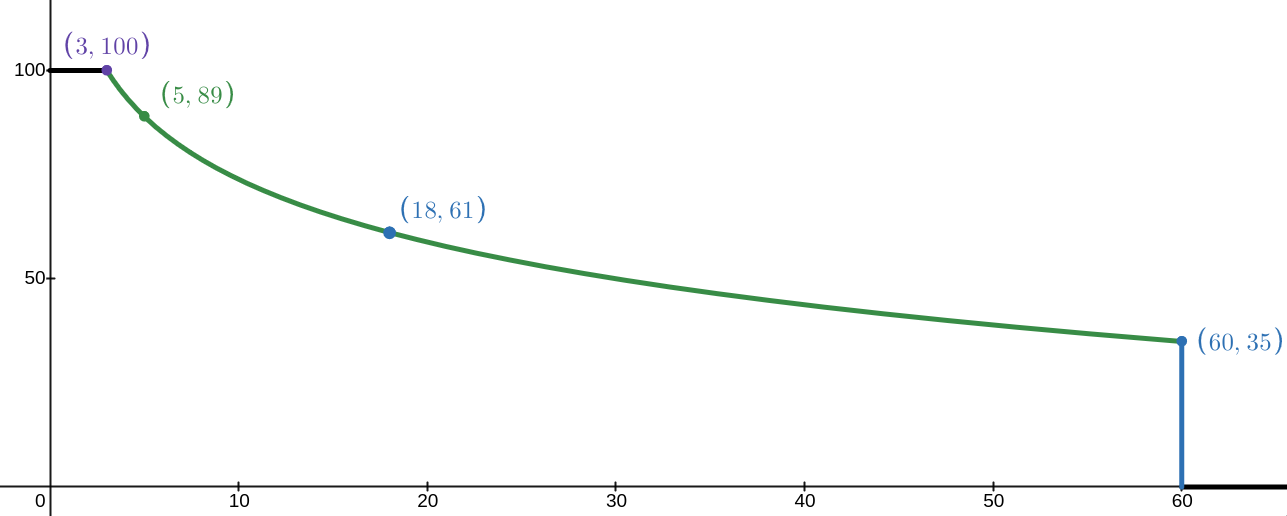
\includegraphics[width=0.95\textwidth]{score_gardendecorations.png}
\end{center}

\section*{Testing Tool}
To facilitate the testing of your solution, we provide a simple tool that you can download.
See ``attachments'' at the bottom of the Kattis problem page.
The tool is optional to use. Note that the official grader program on Kattis is different from the testing tool.

To use the tool, create an input file, such as ``sample1.in'', which should start with a number $N$ followed by a line with $N$ numbers specifying the permutation, and another line with $N$ bits ($0$ or $1$) specifying the initial states of the birds. For example:

\begin{verbatim}
6
1 2 0 4 3 5
1 1 0 0 1 0
\end{verbatim}

For Python programs, say \texttt{solution.py} (normally run as \texttt{pypy3 solution.py}):

    \verb|python3 testing_tool.py pypy3 solution.py < sample1.in|


For C++ programs, first compile it
(e.g. with \texttt{g++ -g -O2 -std=gnu++20 -static solution.cpp -o solution.out})
and then run:

    \verb|python3 testing_tool.py ./solution.out < sample1.in|

\section*{Example}
In the sample, we are given the following permutation of people in the houses:

\begin{figure}[h]
\centering
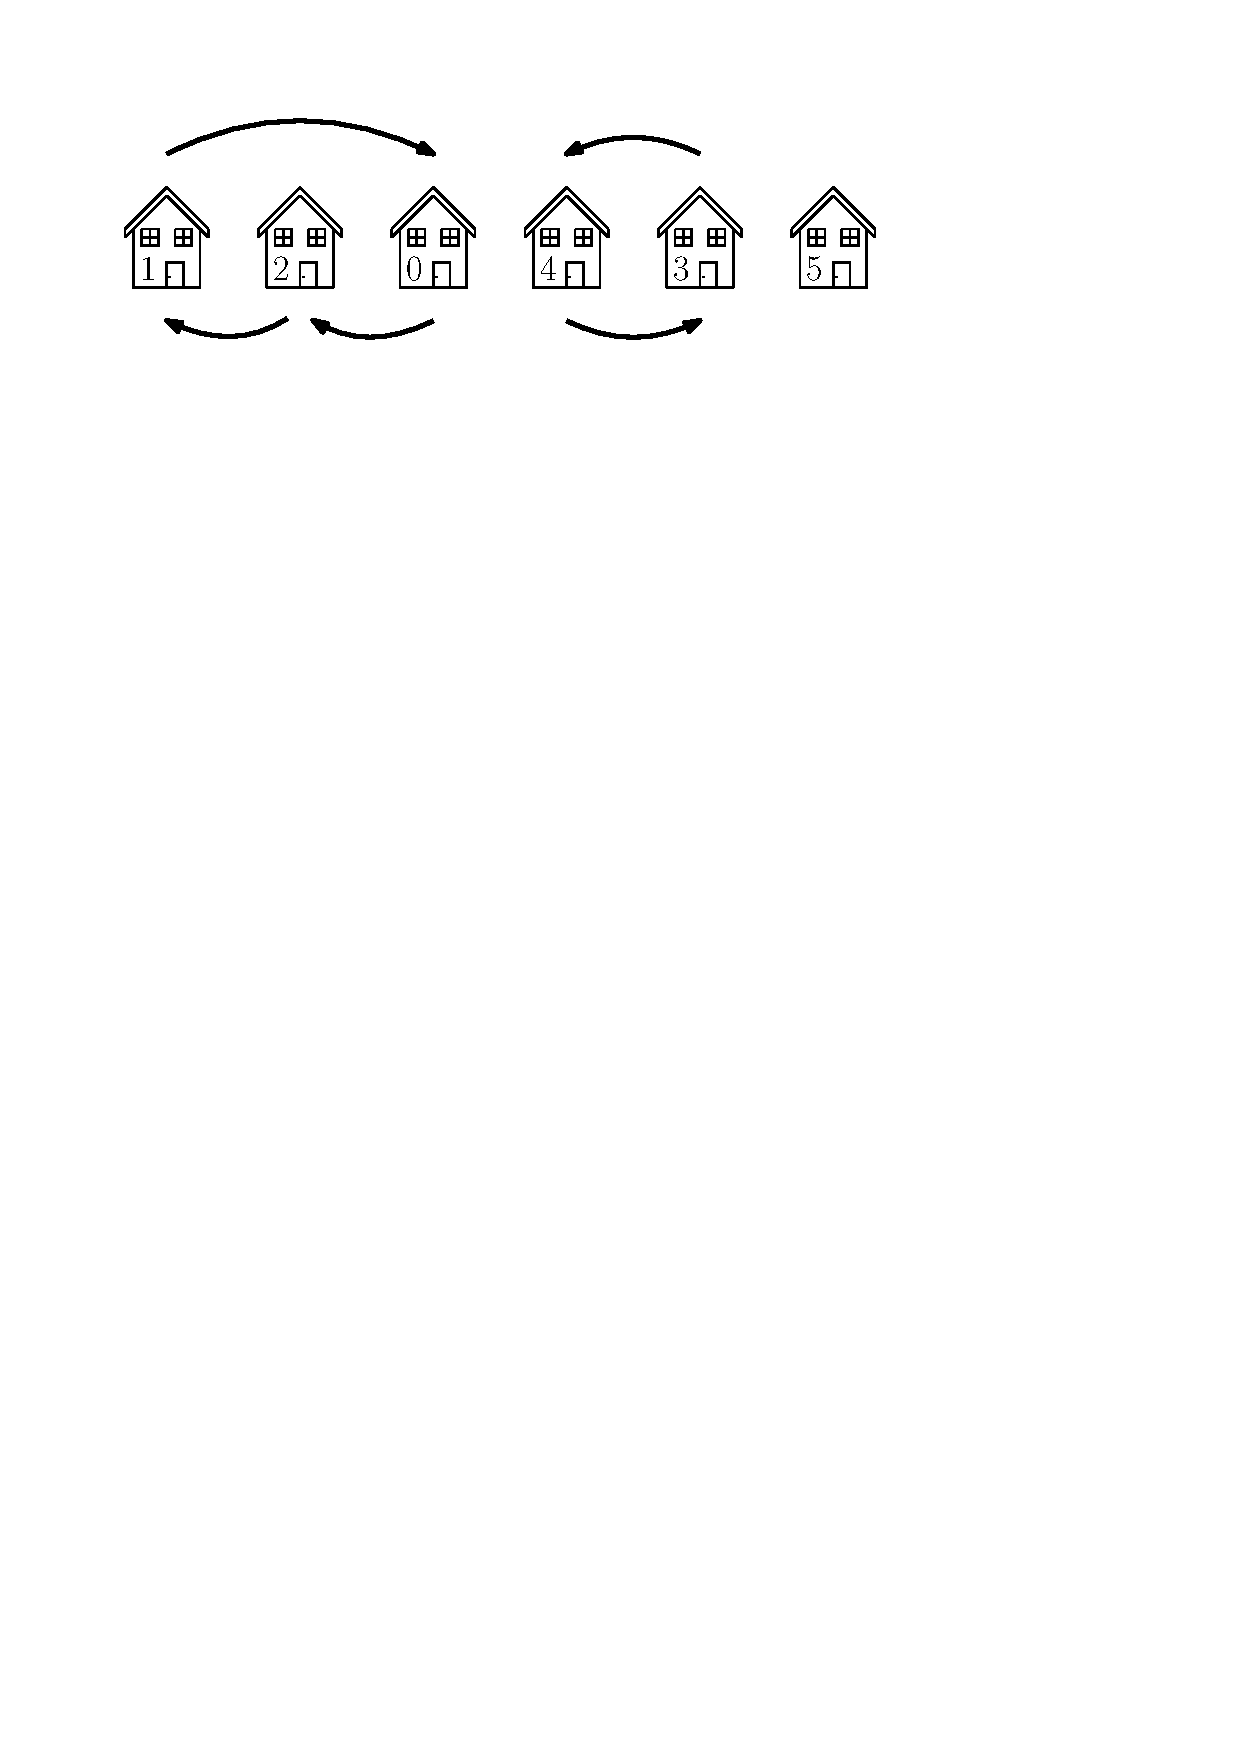
\includegraphics[width=0.95\textwidth]{s1perm}
\end{figure}

The first time the sample program runs (with $w = 0$), it outputs $W = 2$, meaning that Detje will walk along the street two times (and the program will be run two more times).
Before the first walk, the birds in the gardens look like follows:

\begin{figure}[h]
\centering
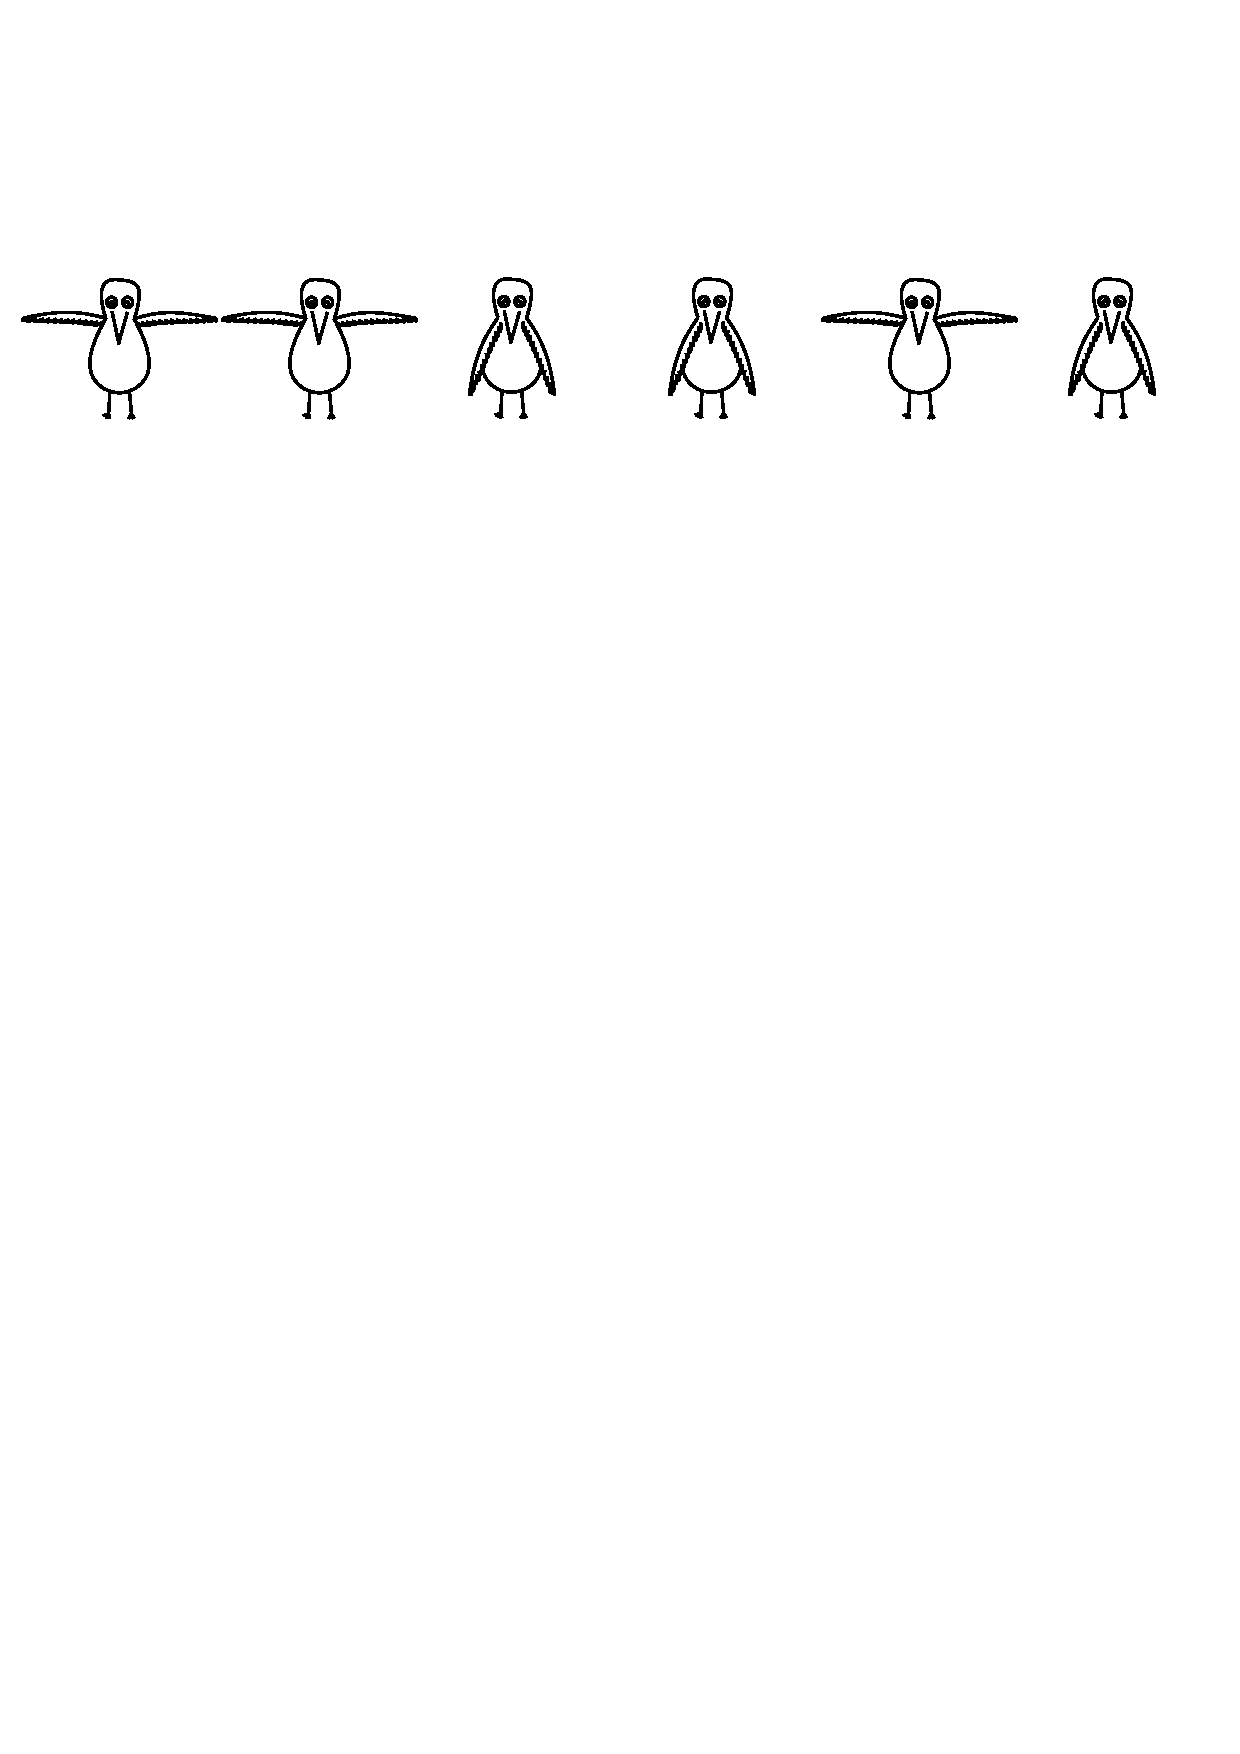
\includegraphics[width=0.95\textwidth]{s1r0}
\end{figure}

Then the program is run with $w = 1$, indicating the first walk of Detje.
She goes through the birds one by one, starting on the left, and possibly changes their state.
The sample program has to output the state of the $i$th bird before we see the $(i+1)$th bird.

After Detje has arrived at school, the states of the birds are:

\begin{figure}[h]
\centering
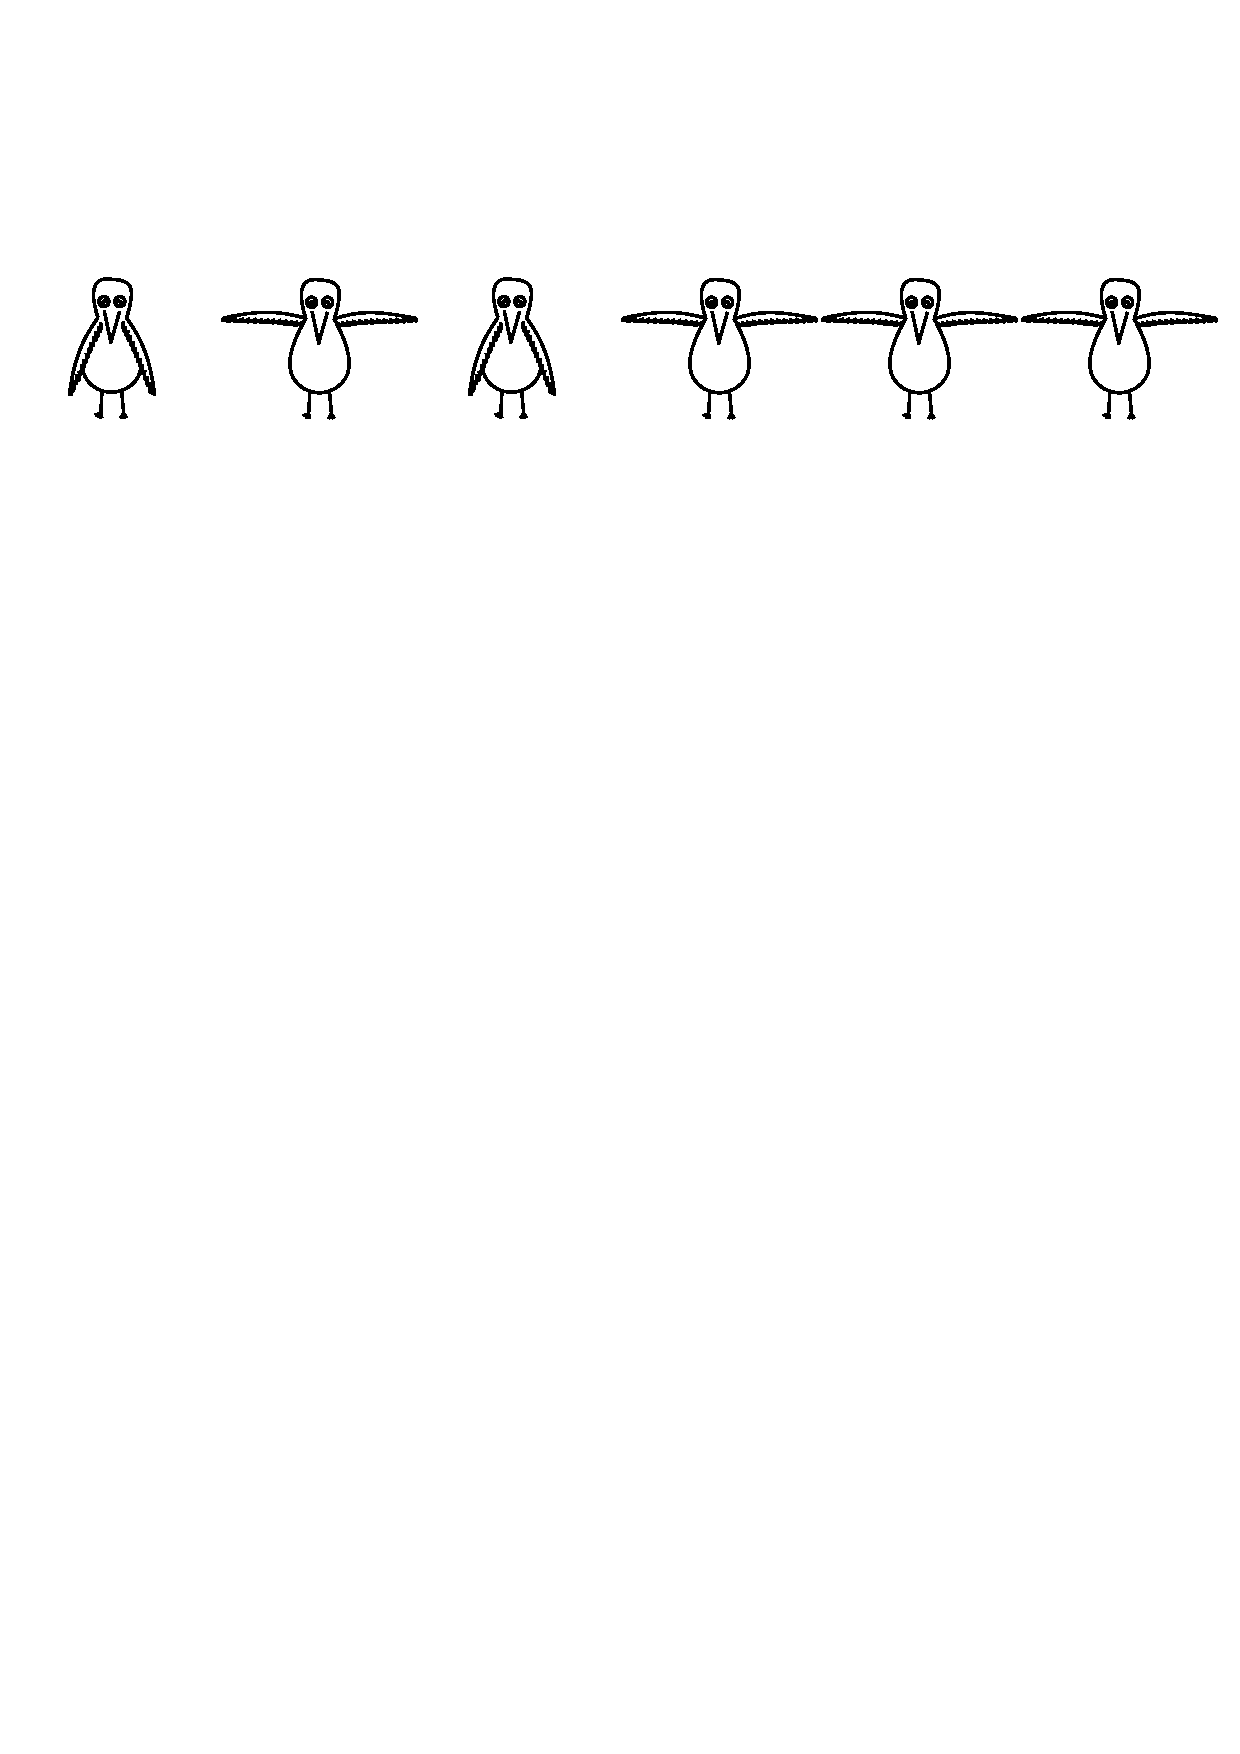
\includegraphics[width=0.95\textwidth]{s1r1}
\end{figure}

In the final run of the program (with $w = 2$),
Detje walks back home from school.
Remember that in this case, she will go through the birds right to left and process them in this order!
This means she needs to determine the state of the $i$th bird before seeing the $(i-1)$th bird.

After she finishes her walk, the birds now look like:

\begin{figure}[h]
\centering
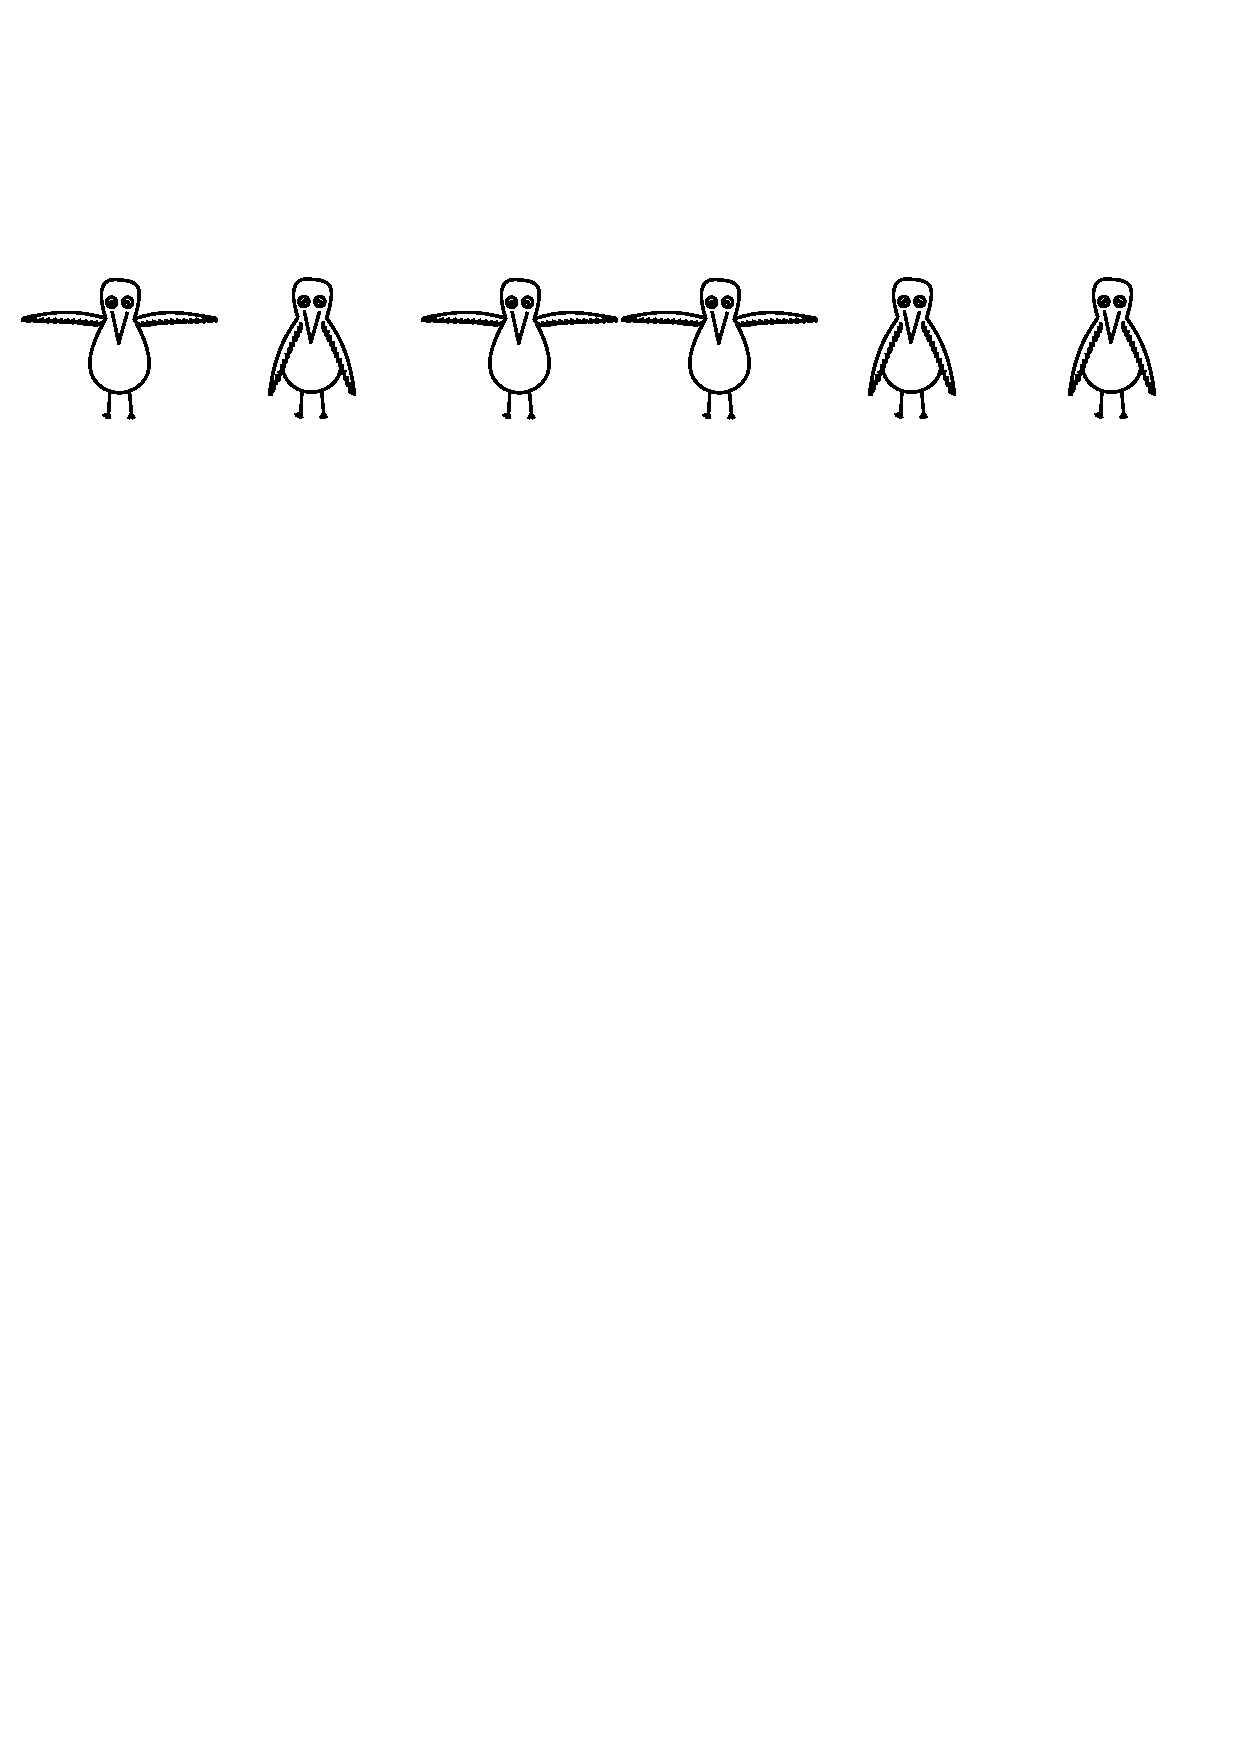
\includegraphics[width=0.95\textwidth]{s1r2}
\end{figure}

Indeed, this is the correct configuration. For example, bird statue $3$ (i.e. fourth from the left) is open (now $b_3 = 1$),
which is correct as person $4$ will be moving there ($a_3 = 4$) and they originally had an open bird statue (originally $b_4 = 1$).



